\section{Aplikacja serwerowa}

Kolejnym etapem pracy było projekt aplikacji serwerowej, która obsługiwałaby zapytania HTTP (\textit{ang. \textbf{H}yper\textbf{t}ext \textbf{T}ransfer \textbf{P}rotocol}) użytkownika oraz zapytania kierowane do bazy danych. Aplikacja została napisana w środowisku Qt. Wybór środowiska nastąpił z kilku powodów. Pierwszym i jednocześnie najważniejszym z nich jest wbudowany moduł obsługi relacyjnych baz danych. Dzięki temu, wykorzystując kilka wysokopoziomowych funkcji można szybko operować na zgromadzonych danych. Ponadto, aplikacja napisana w C++ statystycznie zapewnia większą wydajność niż podobna napisana w języku Java. Ostatnim z powodów jest znajomość tej biblioteki oraz jej metodologii komunikacji wewnętrznej przez autora pracy.

Aplikacja składa się z dwóch głównych modułów: manager'a bazy danych oraz serwera HTTP.

Baza danych składa się z 4 tabel. Są to :

\begin{itemize}
\item Tabela użytkowników
\item Tabela urządzeń
\item Tabela tras
\item Tabela próbek
\end{itemize}

Jako silnik bazodanowy zdecydowano się wykorzystać system SQLite. Stanowi on uproszczony, lecz bardzo wydajny sterownik opierający się na zapytaniach SQL, służący do obsługi relacyjnych baz danych. Kolejną zaletą jest fakt, iż jest on obsługiwany wewnętrznie przez bibliotekę Qt.
Relacje pomiędzy poszczególnymi tabelami bazy danych zostały przedstawione na rysunku \ref{fig:image_soft_db_relations}.

Założenia struktury bazy danych są następujące:

\begin{itemize}
\item Każdy zarejestrowany użytkownik może posiadać więcej niż jedno urządzenie
\item Każde urządzenie może otrzymać opisującą je krótką nazwę
\item Do każdego z urządzeń może być przypisana więcej niż jedna trasa
\item Wpis trasy posiada wpisy o miejscach i czasach ich rozpoczęcia i zakończenia, oraz zbiór przypisanych do niej próbek lokalizacji zbieranych cyklicznie w czasie jej trwania.
\end{itemize}

\begin{figure}[H]
	\centering
	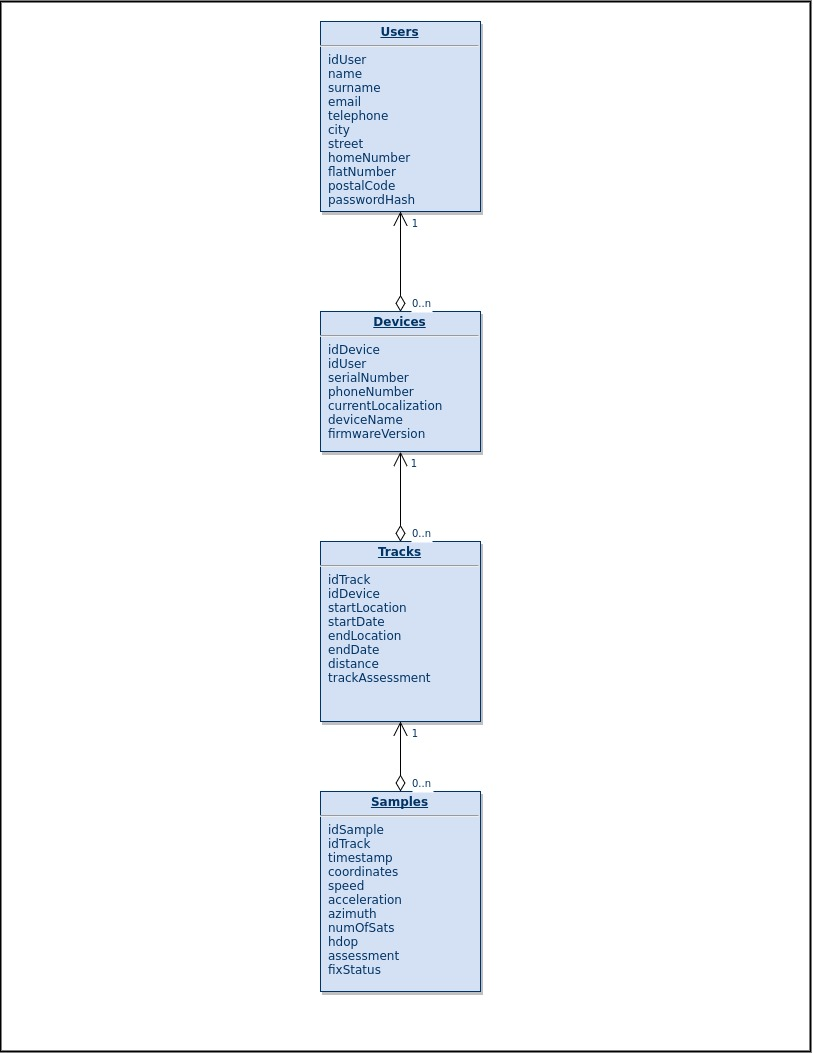
\includegraphics[width=17cm]{img/software/database/Database_relations.jpg}
	\caption{Schemat relacji między tabelami w bazie danych. 
	\\Źródło: Opracowanie własne.}
	\label{fig:image_soft_db_relations}
\end{figure}

Jako serwer HTTP zastosowano bibliotekę QttpServer autorstwa użytkownika supamii \cite{qttpserver}. Została ona napisana pod licencją MIT, co zapewnia swobodę użytkowania i modyfikacji kodu źródłowego, a nawet komercyjne zastosowanie pod warunkiem umieszczenia oryginalnych warunków licencyjnych i informacji o autorze. Biblioteka umożliwia komunikację zarówno poprzez zapytania HTTP typu GET jak i POST. Zapytania te różnią się pomiędzy sobą tym, że w zapytaniu typu GET zmienne przekazywane są jawnie wewnątrz adresu URL, natomiast w zapytaniu typu POST są one ukryte.

Przy pomocy aplikacji, można wykonać następujące operacje:

\begin{itemize}
\item logowanie użytkownika,
\item wylogowanie użytkownika,
\item rejestracja nowego użytkownika,
\item pobieranie danych o użytkowniku z bazy danych,
\item zmianę danych użytkownika,
\item zmianę hasła użytkownika,
\item kasowanie konta użytkownika,
\item dodawanie urządzenia do konta użytkownika,
\item pobieranie listy urządzeń przypisanych do użytkownika,
\item pobieranie informacji o urządzeniu,
\item usuwanie urządzenia z bazy danych,
\item dodawanie nowej trasy do urządzenia,
\item pobieranie listy tras przypisaych do urządzenia,
\item pobieranie informacji o trasie,
\item dodawanie próbek do trasy,
\item zakończanie trasy,
\item usuwanie trasy.
\end{itemize}